% !TEX TS-program = pdflatex
% !TEX encoding = UTF-8 Unicode

\chapter{Feature Engineering} \label{chapter:feature_extraction}

\section{Genes Pre-Selection}

At this stage, there are 168 432 variants present in the dataset. One of the first possible approaches can be to perform feature reduction and follow up with classifiers training. However, with this extreme number of features and comparatively low samples, the likelihood of finding dataset specific patterns that are not scalable to alternative datasets is very high. As such, it is important to find a methodology that is able to adapt to different genotyping data and learn from either more features or samples.

As part of the methodology, and to standardize the approach, a translation of the current datasets from variants to genes was performed. This essentially leaves the data exactly as is, but provides extra information relative to the gene of each variant. This may come across as very little extra information added, but it allows to gather variants in groups, and distinguish with any extracted metric which are the meaningful variants, and the misfits in their group. Nonetheless, the main problem still remains. It is necessary to select which are the important genes.

To do so, two distinctive methods of feature selection are employed. The first one, makes use of prior knowledge of \gls{T2D} genetics, and the second employs regular \gls{GWAS} metrics combined with group information to establish if the genes are relevant or not.

A list of the most relevant genes discovered was obtained from "Genetics of Type 2 Diabetes" \cite{ali2013genetics}. This is not a comprehensive list nor it has all of the variants discovered up to date, but it delivers important information such as the frequency of the risk allele in a population and the Odds Ratio for \gls{T2D}, where it can be seen on table \ref{tab:risk_genes}. 

\begin{table}[]
	\begin{tabular}{|l|l|l|l|>{\centering}p{.9cm}|>{\centering}p{.9cm}|>{\centering}p{.9cm}|l|}
		\hline
		Locus         & Chr & Risk allele frequency & OR (95\%CI)      \\ \hline
		NOTCH2        & 1   & 0.11                  & 1.13 (1.08-1.17) \\ \hline
		PROX1         & 1   & 0.5                   & 1.07 (1.05-1.09) \\ \hline
		IRS1          & 2   & 0.61                  & 1.19 (1.13-1.25) \\ \hline
		THADA         & 2   & 0.92                  & 1.15 (1.10-1.20) \\ \hline
		RBMS1/ITGB6   & 2   & 0.57                  & 1.11 (1.08-1.16) \\ \hline
		BCL11A        & 2   & 0.46                  & 1.08 (1.06-1.10) \\ \hline
		GCKR          & 2   & 0.62                  & 1.06 (1.04-1.08) \\ \hline
		IGF2BP2       & 3   & 0.29                  & 1.17 (1.10-1.25) \\ \hline
		PPARG         & 3   & 0.92                  & 1.14 (1.08-1.20) \\ \hline
		ADCY5         & 3   & 0.78                  & 1.12 (1.09-1.15) \\ \hline
		ADAMTS9       & 3   & 0.81                  & 1.09 (1.06-1.12) \\ \hline
		WFS1          & 4   & 0.27                  & 1.13 (1.07-1.18) \\ \hline
		ZBED3         & 5   & 0.26                  & 1.08 (1.06-1.11) \\ \hline
		CDKAL1        & 6   & 0.31                  & 1.12 (1.08-1.16) \\ \hline
		JAZF1         & 7   & 0.52                  & 1.10 (1.07-1.13) \\ \hline
		GCK           & 7   & 0.2                   & 1.07 (1.05-1.10) \\ \hline
		KLF14         & 7   & 0.55                  & 1.07 (1.05-1.10) \\ \hline
		DGKB/TMEM195  & 7   & 0.47                  & 1.06 (1.04-1.08) \\ \hline
		SLC30A8       & 8   & 0.75                  & 1.12 (1.07-1.16) \\ \hline
		TP53INP1      & 8   & 0.48                  & 1.06 (1.04-1.09) \\ \hline
		CDKN2A/B      & 9   & 0.79                  & 1.20 (1.14-1.25) \\ \hline
		TLE4          & 9   & 0.93                  & 1.11 (1.07-1.15) \\ \hline
		TCF7L2        & 10  & 0.25                  & 1.37 (1.28-1.47) \\ \hline
		HHEX          & 10  & 0.56                  & 1.13 (1.08-1.17) \\ \hline
		CDC123/CAMK1D & 10  & 0.23                  & 1.11 (1.07-1.14) \\ \hline
		KCNQ1         & 11  & 0.61                  & 1.40 (1.34-1.47) \\ \hline
		KCNJ11/ABCC8  & 11  & 0.5                   & 1.15 (1.09-1.21) \\ \hline
		CENTD2        & 11  & 0.88                  & 1.14 (1.11-1.17) \\ \hline
		MTNR1B        & 11  & 0.3                   & 1.09 (1.06-1.12) \\ \hline
		HMGA2         & 12  & 0.1                   & 1.10 (1.07-1.14) \\ \hline
		TSPAN8/LGR5   & 12  & 0.23                  & 1.09 (1.06-1.12) \\ \hline
		OASL/HNF1A    & 12  & 0.85                  & 1.07 (1.05-1.10) \\ \hline
		PRC1          & 15  & 0.22                  & 1.07 (1.05-1.09) \\ \hline
		ZFAND6        & 15  & 0.56                  & 1.06 (1.04-1.08) \\ \hline
		FTO           & 16  & 0.45                  & 1.15 (1.09-1.22) \\ \hline
		HNF1B         & 17  & 0.43                  & 1.12 (1.07-1.18) \\ \hline
		DUSP9         & X   & 0.12                  & 1.27 (1.18-1.37) \\ \hline
	\end{tabular}	\\ \vskip .5cm
	\caption{Collection of chromosome, risk allele frequency and \gls{OR} of 37 risk genes identified for \gls{T2D}. This list was adapted from "Genetics of Type 2 Diabetes" \cite{ali2013genetics}.}
	\label{tab:risk_genes}  
\end{table}

By looking at the \gls{OR} of the genes in the table, it is possible to identify, as previously stated, that all these genes have relatively small values. Besides, these can only explain about 10\% of the observed heritability of \gls{T2D} \cite{ali2013genetics}. The most prominent genes are the KCNQ1 and TCF7L2, them being the only ones with \gls{OR} higher than 1.3. The \gls{OR} is a metric indicative of association between a variable and an outcome of interest. Given the two-by-two frequency table \ref{tab:frequency_table} the \gls{OR} is calculated through:
\begin{equation}
OR = \frac{a \times d}{b \times c} 
\end{equation}

\begin{table}[h]
	
	\begin{tabular}{|c|c|c|>{\centering}p{.9cm}|>{\centering}p{.9cm}|>{\centering}p{.9cm}|c|}
		\hline                
		 & Diseased & Healthy\\ 
		\hline
		exposed & a & b\\
		not-exposed & c & d \\
		\hline
	\end{tabular} \\ \vskip .5cm
	\caption{\gls{OR} two-by-two frequency table.}
	\label{tab:frequency_table}  
\end{table}

The closer \gls{OR} is to one, the more indicative it is that the exposure does not affect the odds of the outcome. If it is higher, the exposure is associated with high odds for the outcome, and vice-versa. As such, and as it can be seen by the known \gls{T2D} risk genes, these are not linked with moderate risks \cite{szumilas2010explaining}. However, by using them together in a classifier, some non-linear relationships might be picked up, that are not clear with only \gls{OR}.

Since the association between genes and variants was previously performed, the process of identifying the risk ones is very straightforward. However, since there was only data from \gls{WES}, there are some risk genes that were not picked up in the current dataset. Out of the 37 genes, 18 were present, including some with higher \gls{OR} such as KCNQ1 and DUSP9, but other also important ones like TCF7L2 and CDKN2A/B weren't. However, since one of the goals of this study is to also try and find new markers, it is necessary to include other genes. To do so, the standard association \textit{Pearson's} $\chi^2$ test is going to be used. It is then possible to group it's results to find more meaningful regions or genes. 
Even more so, since this data is nominal, the \textit{Pearson's} $\chi^2$ test is one of the most adequate for this situation. The Fisher test could also be applied, but as it can be seen further down, one metric is sufficient.

\begin{figure}[h]
	\centering
	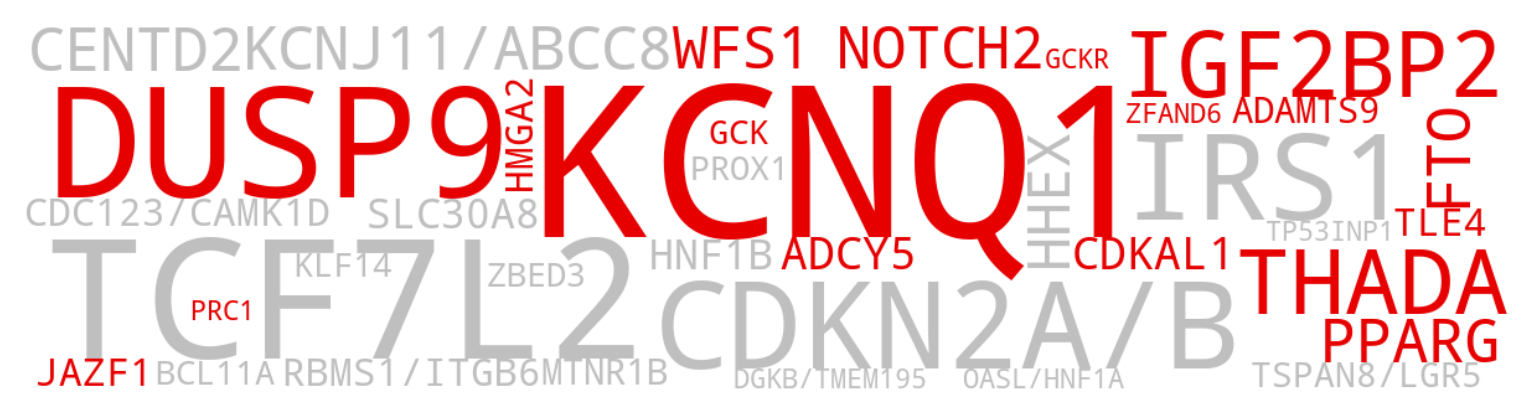
\includegraphics[width=\textwidth]{../images/feature_extraction/genes_wordcloud.png}
	\caption{List of risk genes which were attempted to be found in the dataset. Genes present in the data are red coloured, and the remainders are silver. The bigger the size of a word, the bigger it's known \gls{OR} to \gls{T2D} according to "The genetic architecture of type 2 diabetes" \cite{fuchsberger2016genetic}.} 
	\label{fig:genes_wordcloud}
\end{figure}

\begin{figure}[h]
	\centering
	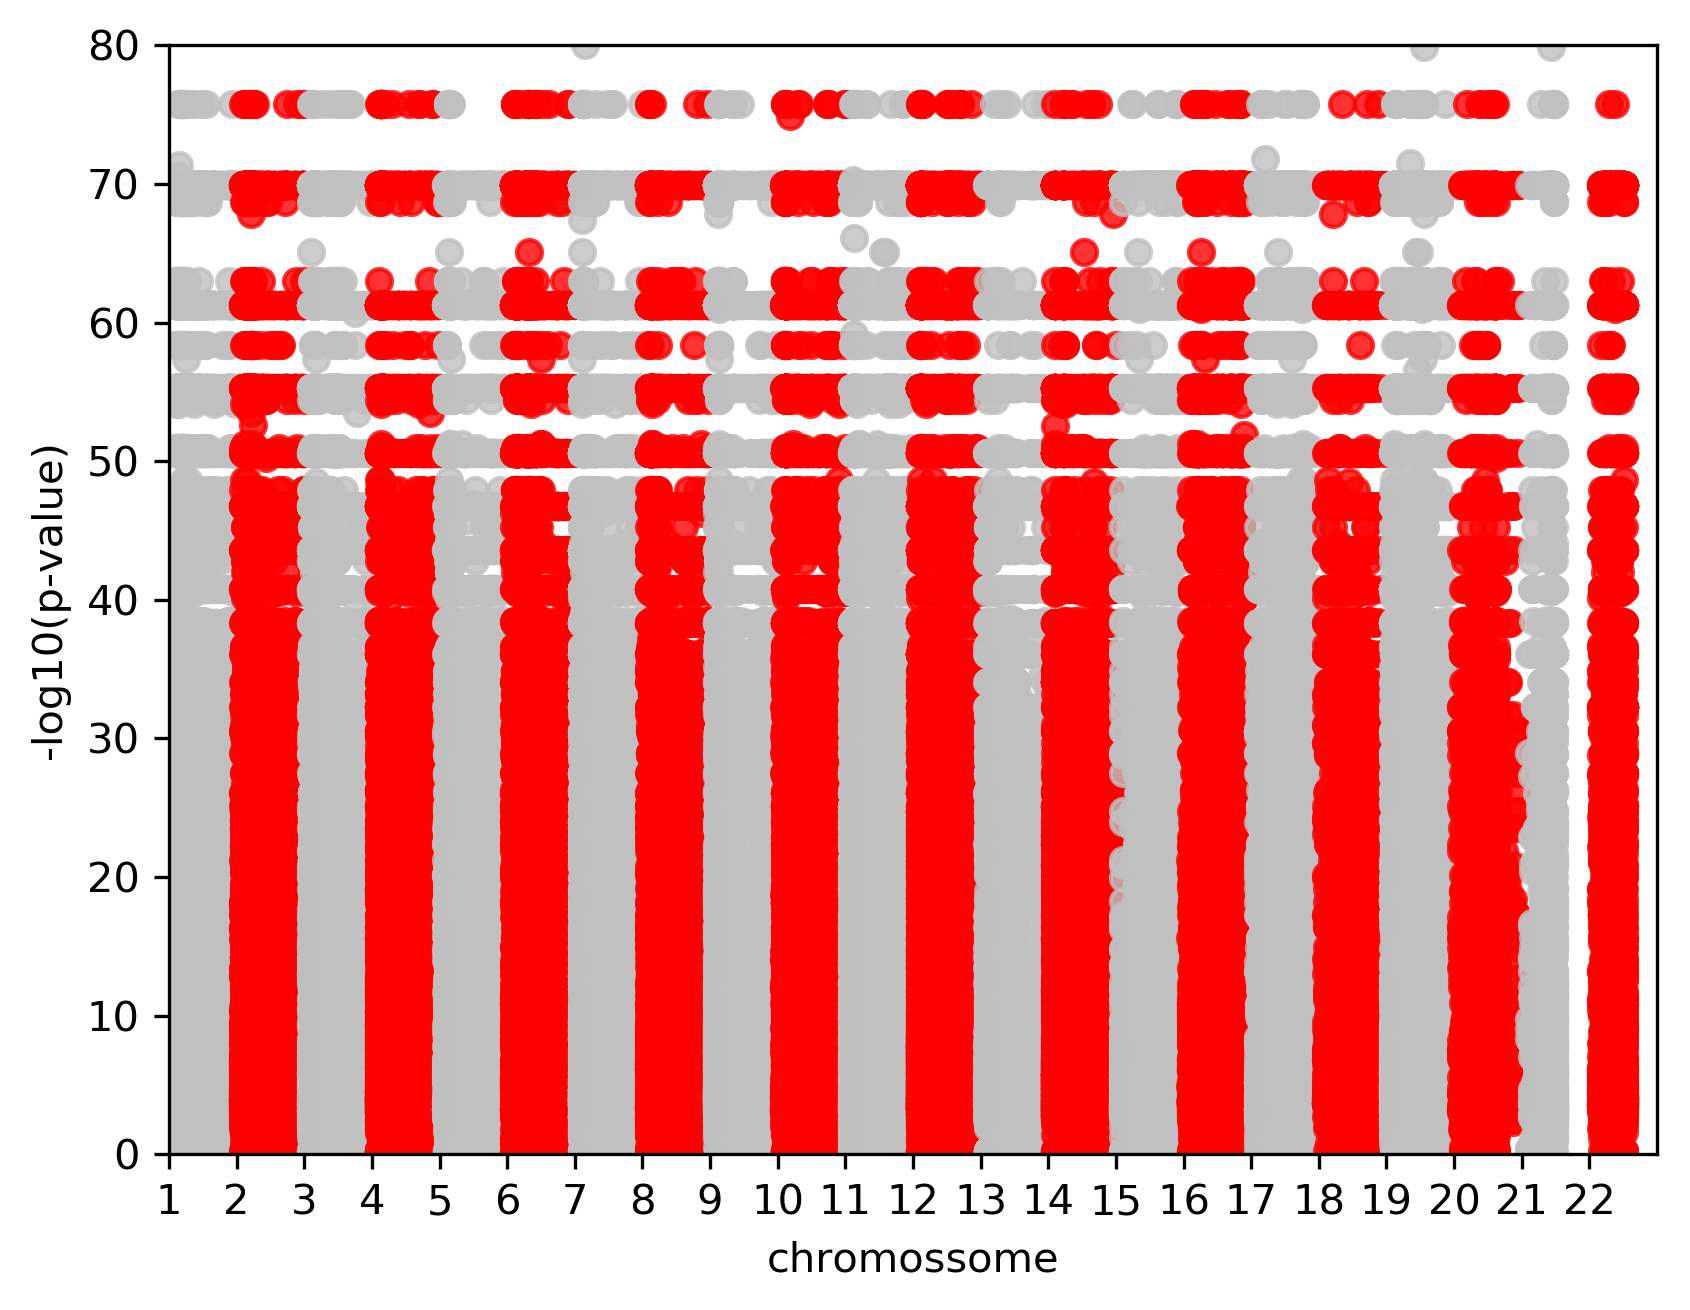
\includegraphics[width=\textwidth]{../images/feature_extraction/normality.png}
	\caption{$-log10(p-value)$ of the D'Agostino's K-squared test for normality plotted against each variant's position in the chromosome.} 
	\label{fig:normal}
\end{figure}

Before testing the variables, it is first necessary to test if they follow a normal distribution. Since Shapiro-Wilk normality test is not deemed accurate for over 50 samples, D'Agostino's K-squared test was used to test it, since it is the one performed by the "normaltest" function of the statistics python module Scipy. The test was applied to every variable, and the $-log_{10}(p-value)$ was calculated and plotted against each variant's position in the genome, as it can be seen on figure \ref{fig:normal}. Since the $-log_{10}(0.05) = 1.3$, and most of the values hugely surpass it, we assume all variants follow a normal distribution.

The next step, is to actually apply the \textit{Pearson's} $\chi^2$ test. This was performed in a similar way to the normality test. After it, we can clearly see in the figure \ref{fig:chi} that some regions show higher correlation to the classes of \gls{T2D} and healthy. However, by only choosing variants directly applying this metric, noisy or incorrectly genotyped are still going to be picked up.  

\begin{figure}[h]
	\centering
	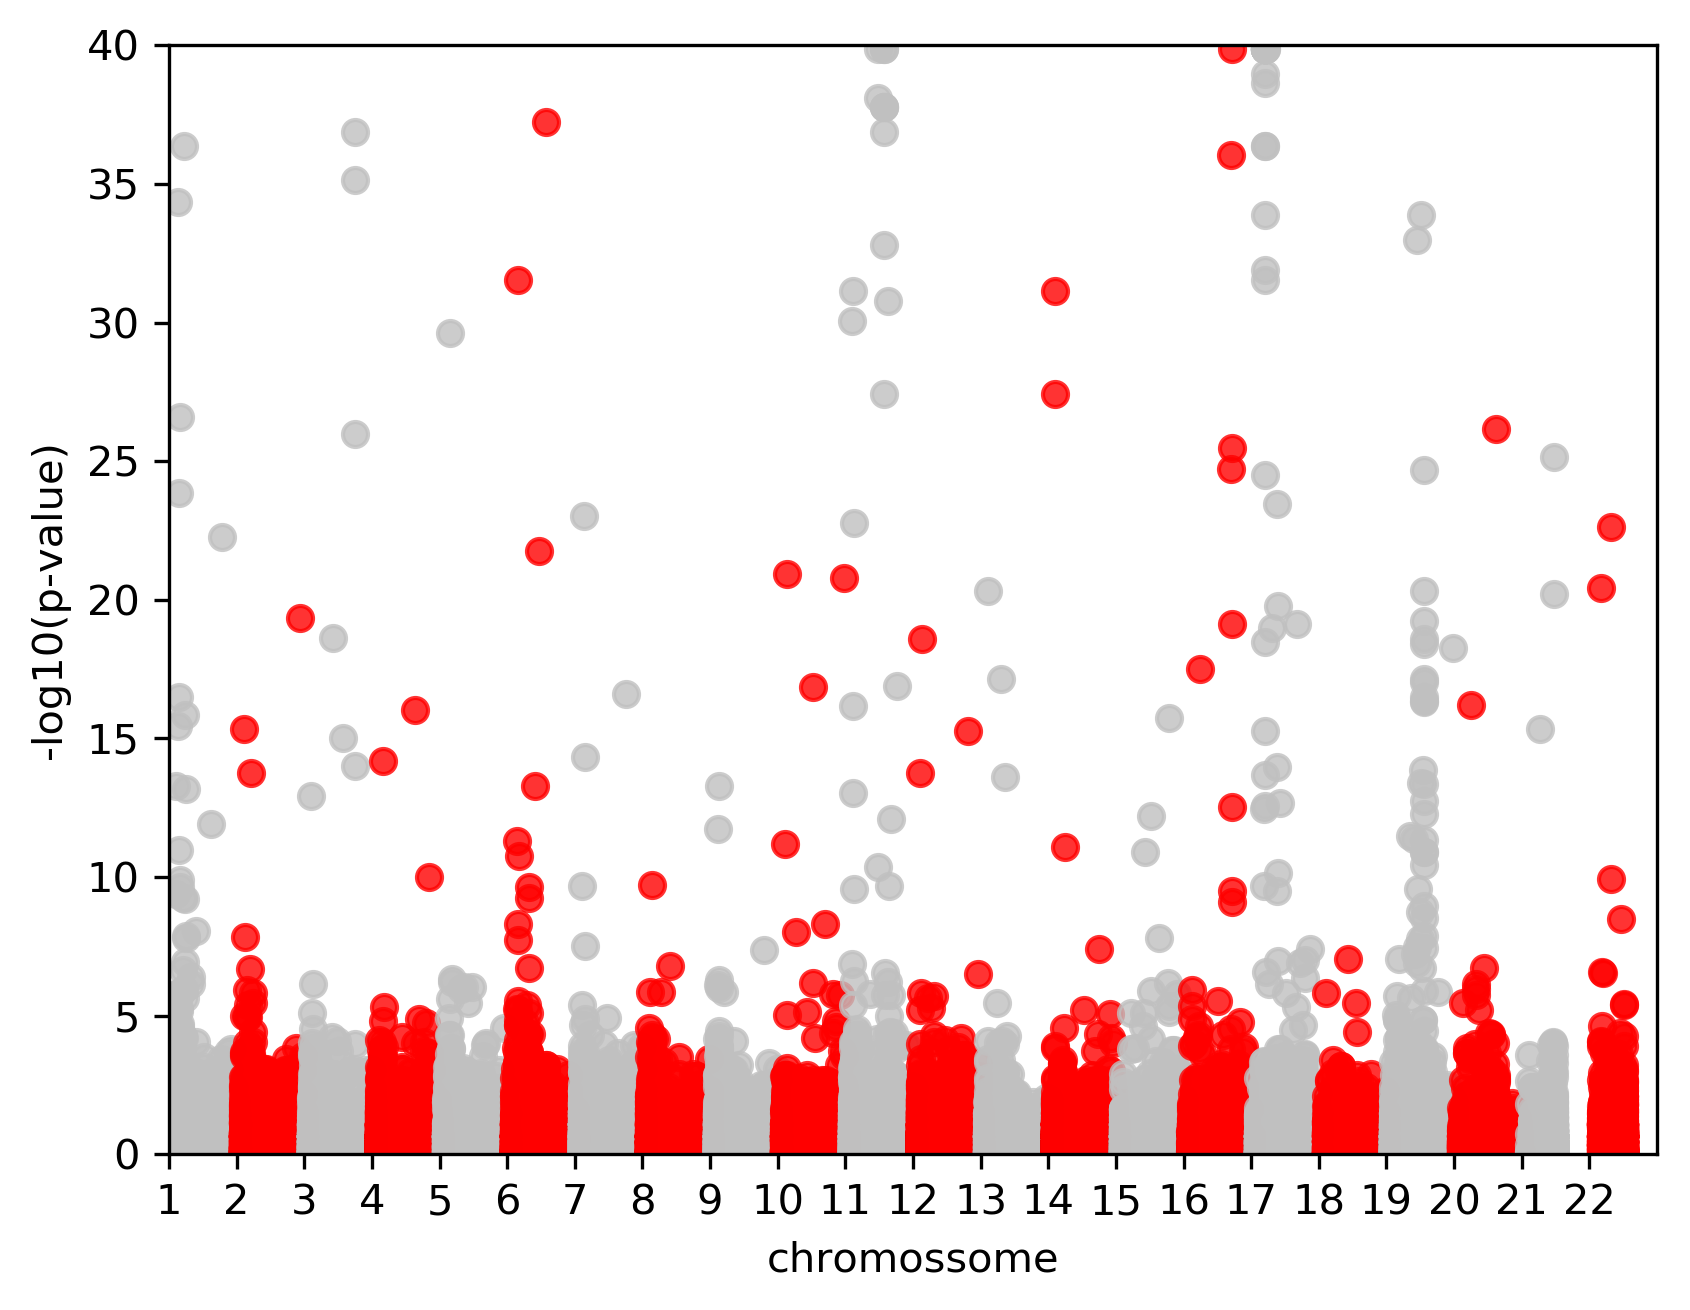
\includegraphics[width=\textwidth]{../images/feature_extraction/manhattan.png}
	\caption{$-log10(p-value)$ of the \textit{Pearson's} $\chi^2$ test plotted against each variant's position in the chromosome.} 
	\label{fig:chi}
\end{figure}

Normally, to solve this issue, a Bonferroni correction is applied. If multiple tests are performed, the probability of a rare occurrence increases, and with it the likelihood of incorrectly rejecting a null hypothesis. As such, the $\alpha$ probability that a null hypothesis is rejected changes according to:
\begin{equation}
pi \leq \frac{\alpha}{m}
\end{equation}
, where m is the number of tests completed. Instead of using it, a more region centred approach was used, that flags every gene where the average of every variant's p-value is less that 0.05. From it, 120 genes were selected, which greatly reduces the previous gigantic amount of features. By adding up the 18 identified \gls{T2D} risk genes, the dataset ends up with 138 genes. 

\section{Feature Extraction}

At this point, the dimension of the dataset has been greatly reduced, but it still contains data of variants that can single-handedly over fit the Machine Learning models, especially since they are very likely to be overly correlated to both classes. So, rather than using them straight away, we can apply dimensionality reduction techniques, and by doing so, combine all the information and genotypes of one gene into a single dimension. Besides this, it is also possible to extract variance and mean of genotypes for each sample, to extract even more information.

The first dimensionality reduction method applied is the Principal Component Analysis. Since in this case, the projection only needs to be performed to one dimension, the only component that matters is the first one. For every single gene, this method is applied, which returns a vector of the first Principal Component, thus combining all the variants of each gene. The same strategy was applied with Linear Discriminant Analysis. This method assumes that the features are normally distributed, which was already tested beforehand. These two extracted features for each gene already capture most of the information contained by them, but to improve it even further, the mean and variance of genotypes by sample were also added.

Ultimately, the final dataset will be a combination of these 4 extracted features for each one of the originally selected 138 genes, which totals 552 features. These are named as "gene\_method", so it is possible to identify the most relevant
genes and feature extraction methods for each classifier.


\section{Feature Reduction} \label{s:fr}

To perform feature selection, we make use of an Extremely Randomized Trees ensemble (Extra-Trees for short), and it's ability to output which are the most important features. This classifier is an ensemble of Decision Trees, with the particularity of being much faster to train than Random Forests. These are among the most powerful Machine Learning algorithms available. The actual results and other metrics are not entirely relevant at this point, since only feature selection is being performed. This method can be seen in figure \ref{fig:tree_rules}, which reflects the nodes of a simple decision tree applied to the final version of the dataset, with Gini impurity measure and the classes labelled as control for the healthy group, and target for the \gls{T2D} affected group.

To make use of this selection method, 1000 Extra-Trees classifiers were trained with the 552 features. For every classifier, the top 100 most important features were selected and counted. Using these counts, it is then possible to gather the frequency of which features are the most important when building an Extra-Trees classifier.

\begin{figure}[h]
	\centering
	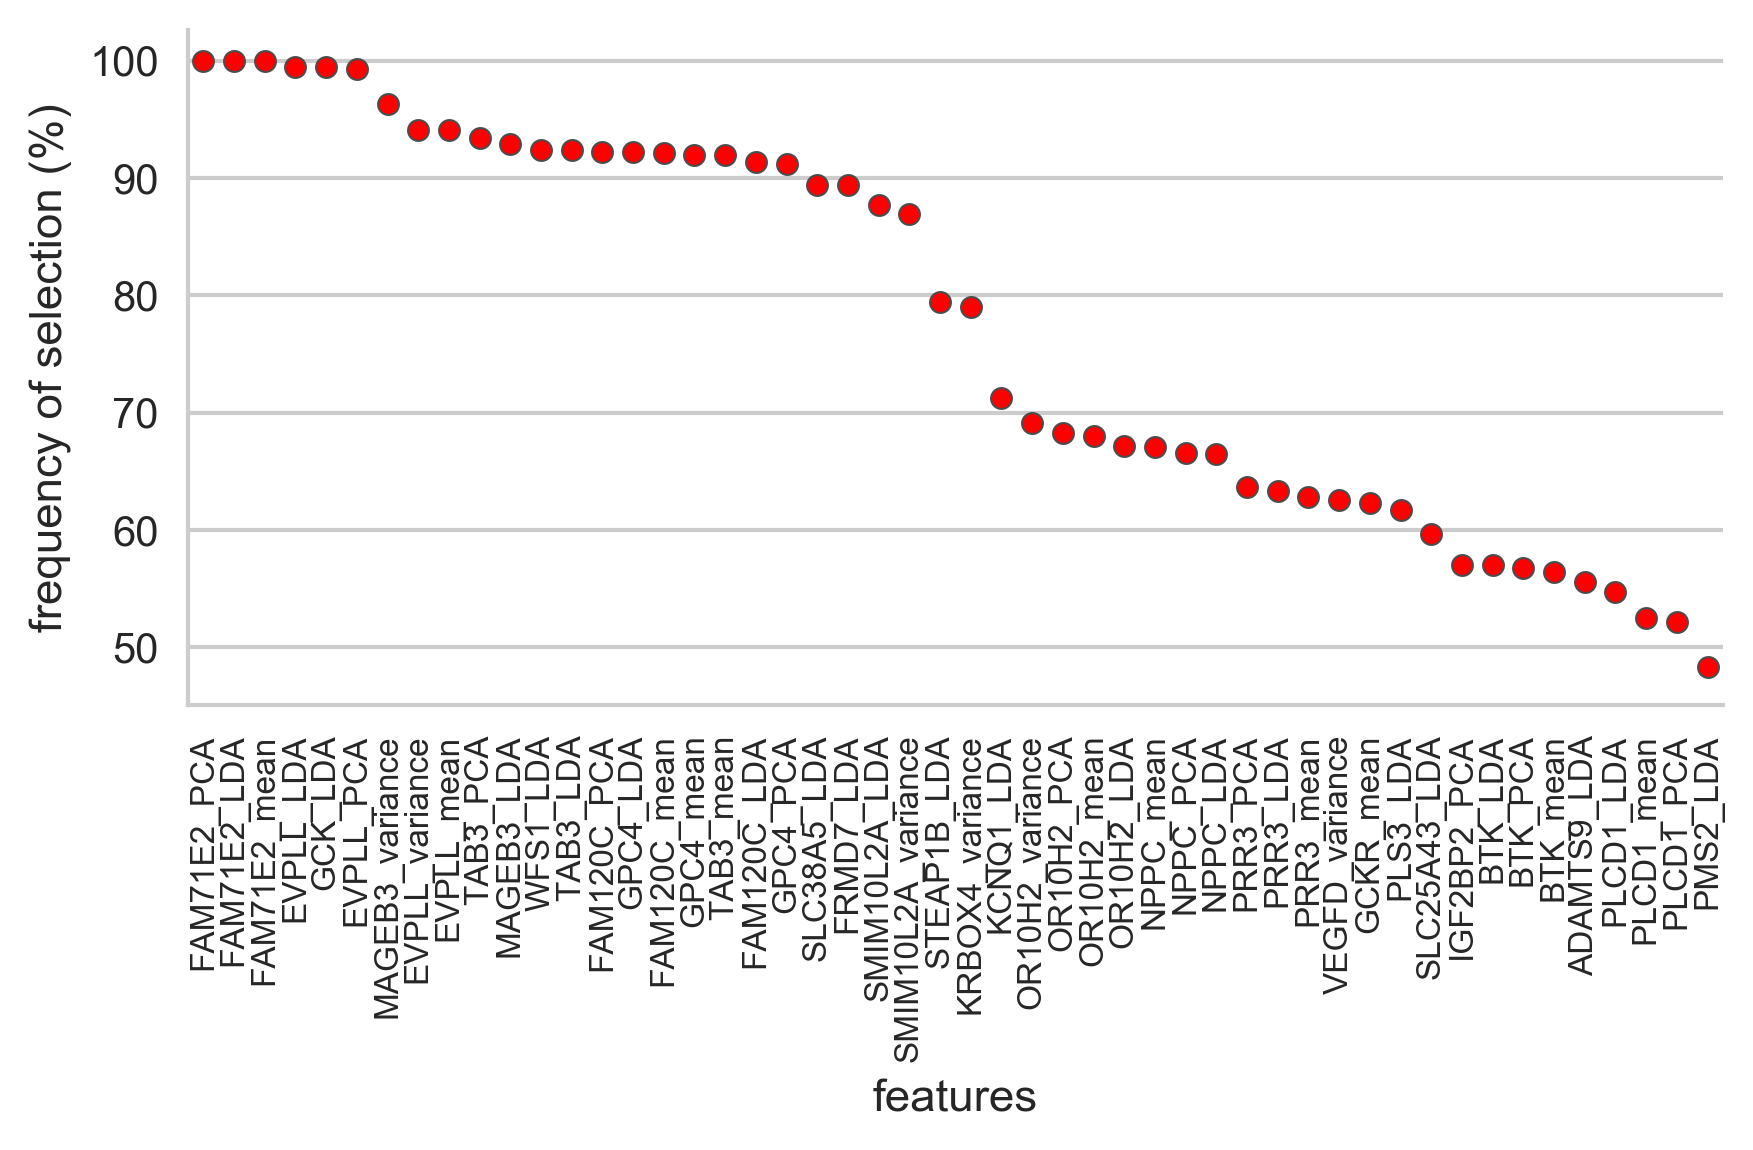
\includegraphics[width=\textwidth]{../images/feature_extraction/top50_features.png}
	\caption{Frequency of times a feature was on the top 100 important features for each of
		the 1000 Extra-Trees classifiers trained. Top 50 features displayed. } 
	\label{fig:top_features}
\end{figure}

From this test, features with over 50\% frequency were selected, which amounts to a total of 49 features displayed on figure \ref{fig:top_features}. Furthermore, from the selected features, we can verify that 25 genes are present, 6 of them already known for being linked to higher risk of T2D. Those risk genes are GCK, WFS1, KCNQ1, GCKR, IGF2BP2 and ADAMTS9. 


\begin{table}[h]
	\begin{tabular}{|l|l|l|>{\centering}p{.9cm}|>{\centering}p{.9cm}|>{\centering}p{.9cm}|l|}
		\hline
		Gene          & Chromosome & Most Related Disease               \\ \hline
		FAM71E2       & 19 & No results shown    \\ \hline
		EVPLL         & 17 & Prostate Cancer  \\ \hline
		GCK			  & 7  & Maturity-Onset Diabetes of the young, Type 2 \\ 	
		        	  &    & Diabetes Mellitus  \\ \hline
		MAGEB3		  & X  & Melanoma   \\ \hline
		TAB3   		  & X  & Different Types of Cancer \\ \hline
		WFS1   		  &    & Wolfram Syndrome-1\\ 
					  &    & Diabetes Mellitus \\ \hline
		FAM120C   	  &	X  & Autism \\ \hline
		GPC4  		  &	X  & Simpson-Golabi-Behmel Syndrome\\ \hline
		SLC38A5  	  & X  & Pancreatic Ductal Adenocarcinoma\\ \hline
		FRMD7	  	  & X  & X-Linked Infantile Nystagmus\\ \hline
		SMIM10L2A  	  & X  & No results shown\\ \hline
		STEAP1B		  & 7  & Prostatitis \\ \hline
		KRBOX4		  & X  & Wilms Tumor 1 \\ \hline	
		KCNQ1		  & 11 & Long Qt Syndrome 1 \\
					  &    & Diabetes Mellitus \\ \hline	
		OR10H2		  & 19 & No results shown \\ \hline	
		NPPC		  & 2  & Congestive Heart Failure \\ \hline	
		PRR3		  & 6  & No results shown \\ \hline	
		VEGFD		  & X  & Different Types of Cancer \\ \hline	
		GCKR		  & 2  & Maturity-Onset Diabetes of the Young \\
					  &    & Diabetes Mellitus \\ \hline
		PLS3		  & X  & Osteoporosis \\ \hline	
		SLC25A43	  & X  & Breast Cancer \\ \hline	
		IGF2BP2		  & 3  & Diabetes Mellitus, Noninsulin-Dependent \\ \hline	
		BTK			  & 22 & Agammaglobulinemia, X-Linked \\ \hline
		ADAMTS9		  & 3  & Peters-plus syndrome \\
				      &    & Different Types of Cancer\\
				      &    & Body Mass Index Quantitative Trait Locus 11 \\ \hline	
		PLCD1    	  & 3  & Nail Disorder, Nonsyndromic Congenital, 3 \\ \hline			
	\end{tabular}\\ \vskip .5cm
	\caption{Ordered list of risk genes discovered and their most related diseases according to $www.malacards.org$ , a human disease database.}
	\label{tab:top_genes}  
\end{table}

\begin{sidewaysfigure}[h]
	\centering
	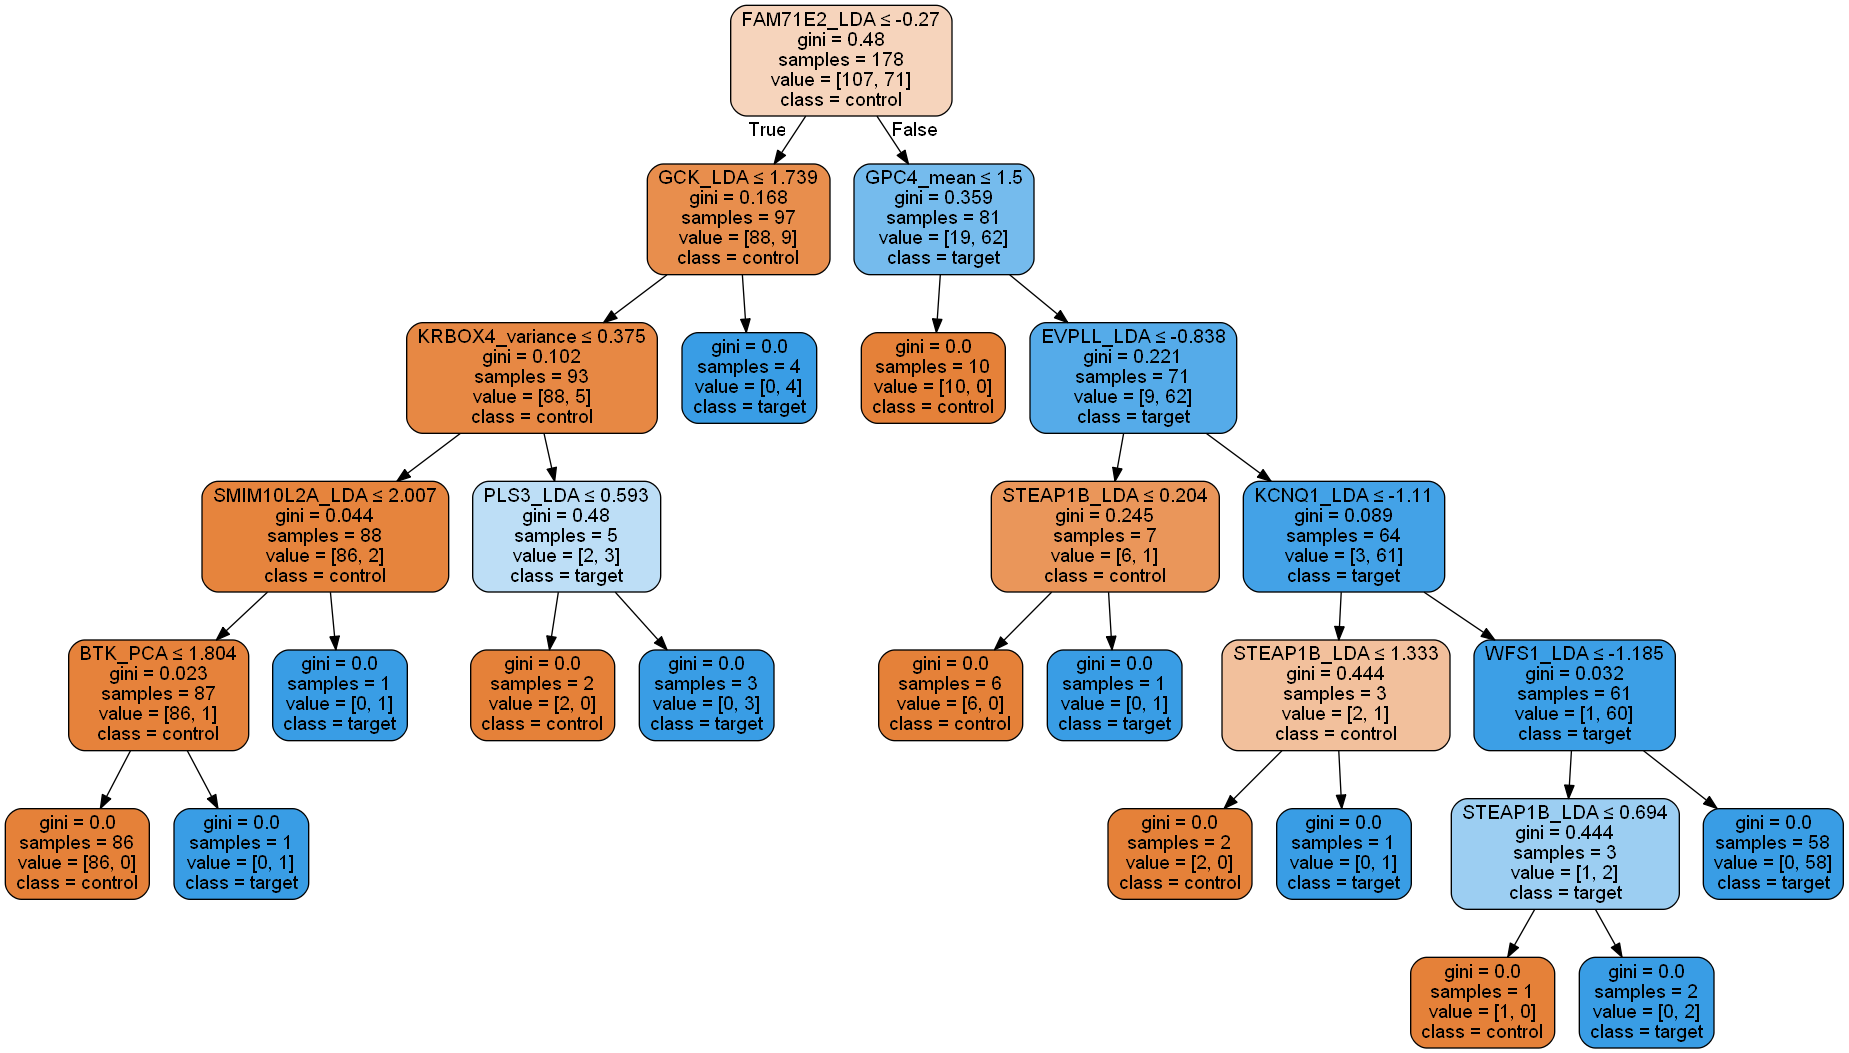
\includegraphics[width=\textwidth]{../images/feature_extraction/tree_rules.png}
	\caption{Decision Tree built with the dataset that contains all the features from the combined genes.} 
	\label{fig:tree_rules}
\end{sidewaysfigure}